\chapter{Detailed System Design}
\vspace{-2em}
\section{Hardware}


This system consists of multiple interconnecting components that will be discussed in detail in this section, namely:
\begin{itemize}
	\item ESP32-S2
	\item Sensiron Sen55
	\item Senseair K30
	\item SD-card adapter
	\item ATGM336H GPS module
	\item Power bank	
\end{itemize} 




\subsection{ESP32-S2}

\begin{figure}[!htb]
	\centering
	\includegraphics[width=0.4\linewidth]{body/fig/s2_mini}
	\caption{ESP32-S2 mini}
	\label{fig:s2mini}
\end{figure}


\noindent
The module used is the ESP32-S2 mini by WEMOS/Lolin. This module features thirty seven digital pins, three SPI interfaces with two of them fully available, two i2c buses, dual hardware UARTs, a built-in WiFi radio with antenna on board. The board runs on 3.3v power, but has an onboard voltage regulator that works on 5V. Although the board supports multiple i2c devices, it was chosen to connect both devices to one bus since they have different addresses. This also alleviates some space in memory by not having another initialisation of the i2c library instance. The board features an ultra low power co-processor capable of waking up from i2c interrupts, this could be used if deploying for longer durations. The main processor is an {Xtensa\textregistered}  32 bit Single Core Microprocessor that operates at up to 240MHz. Should this device be deployed with only internet capability in a data sensitive environment it also features cryptographic hardware accelerators. The board features native support for USB and does not need a serial bus bridge, making debugging much easier. It is also rated for extreme conditions, capable of working at up to 120 degrees Celsius\cite{wemos2021s2mini}.


\subsection{Sensirion SEN55}
\begin{figure}[!htb]
	\centering
	\includegraphics[width=0.7\linewidth]{body/fig/SEN5x}
	\caption{Sensirion SEN55}
	\label{fig:sen5x}
\end{figure}
\noindent
This sensor provides Particulate Matter, Relative Humidity, Temperature, VOC Index and NOx Index outputs.
It is produced by Sensirion and uses a ACES 51452-006H0H0-001 connector interface to connect. It communicates using the i2c bus and has a library available to use to read its values, however, the NOx and VOC outputs are in the format of an index and the raw values are available but the conversion algorithm is proprietary, the index is thus used. The board uses 5v power as its VCC but communicates over i2c at 3.3V common voltage. The 5V is provided straight from the power bank in this use case.
For the readings from the sensor, the particulate matter, relative humidity and temperature values are available immediately, with the VOC value following shortly behind. For the NOx and VOC values to be reliable, the sensor needs to be in operation for 1 hour for VOC and 6 hours for NOx. For extended use, as would be the case in the taxi rank, the sensor has a learning function on the VOC and NOx index, which is set by default as 12 hours. From this the sensor will estimate the mean gain for the previous 12 hours. The device also features a self cleaning mode, this runs once a week.


\subsection{Senseair K30}
\begin{figure}[!htb]
	\centering
	\includegraphics[width=0.6\linewidth]{body/fig/k30fr}
	\caption{Senseair K30 FR}
	\label{fig:k30fr}
\end{figure}
The Senseair K30 FR module is an NDIR $ CO_2 $ sensor with 5000 ppm sensing range and an accuracy of 3\%. It has a rate of measurement of 2Hz and a response time of 2 seconds, but since we are not using a gas tube, the diffusion time is 20 seconds which should be appropriate for the application. The sensor has a few ways to interface with the microcontroller, it features two analog outputs of 0 to 5V and 0 to 10V respectively representing 0 to 5000 ppm. It also features UART utilizing the MODBUS protocol as well as i2c communication. The sensor runs on 5 to 14V for power and has a dedicated input for the communications voltage, allowing the microcontroller to communicate at 3.3 or 5V depending on the model. The sensor communication is done using i2c and there is a detailed document by Sensair describing the protocol. The module also features the ability to change its address, this persists through power down, this negates the issue of having two sensors with the same address conflicting in the case of default addresses. 
\begin{figure}[!htb]
	\centering
	\includegraphics[width=0.7\linewidth]{body/fig/i3ck30}
	\caption[i2c for K30]{The i2c lines SDA and SDL are defined on the factory connector as well as the G+ and G0 representing VCC 5V in this case and ground along with DVCC representing the 3.3V communications voltage.}
	\label{fig:i3ck30}
\end{figure}

 
\subsection{SD-card adapter}



\subsection{ATGM336H GPS module}


\subsection{Power bank}
%The ESP32-S2 is capable of multiple STA and AP modes, including simultaneous broadcasting over ESP-NOW and WiFi. This is needed to be able to have the 2 ESP boards communicate and the base station be able to send the data to a database.
%\subsection{SD - interface}
%The SD card interface was done using SPI. The module was hard soldered to a micro SD to SD card adapter. These pins were then soldered to the ESP32's SPI and 3.3V pins.
%The FS, SD and SPI libraries from Espresiff were used to interface with the already formatted micro SD card.



%
%\subsection{Sensors}
%\subsubsection{$\mathrm{CO_2}$}
%{\color{red} \huge Insert docs you made while working with them}
%
%% why was it chosen
%
%
%\subsubsection{PM, $\mathrm{NO_x}$, VOC, Temperature, Humidity}
%\noindent
%The main ESP referenced as the Base station, will be connected periodically to the internet to send the data it collects to the database of choice. 


\pagebreak
\subsection{Software/Firmware implementation}
\subsubsection{Overview}
%{\color{red} \huge Insert flowchart}

\begin{figure}[!htb]
	\centering
	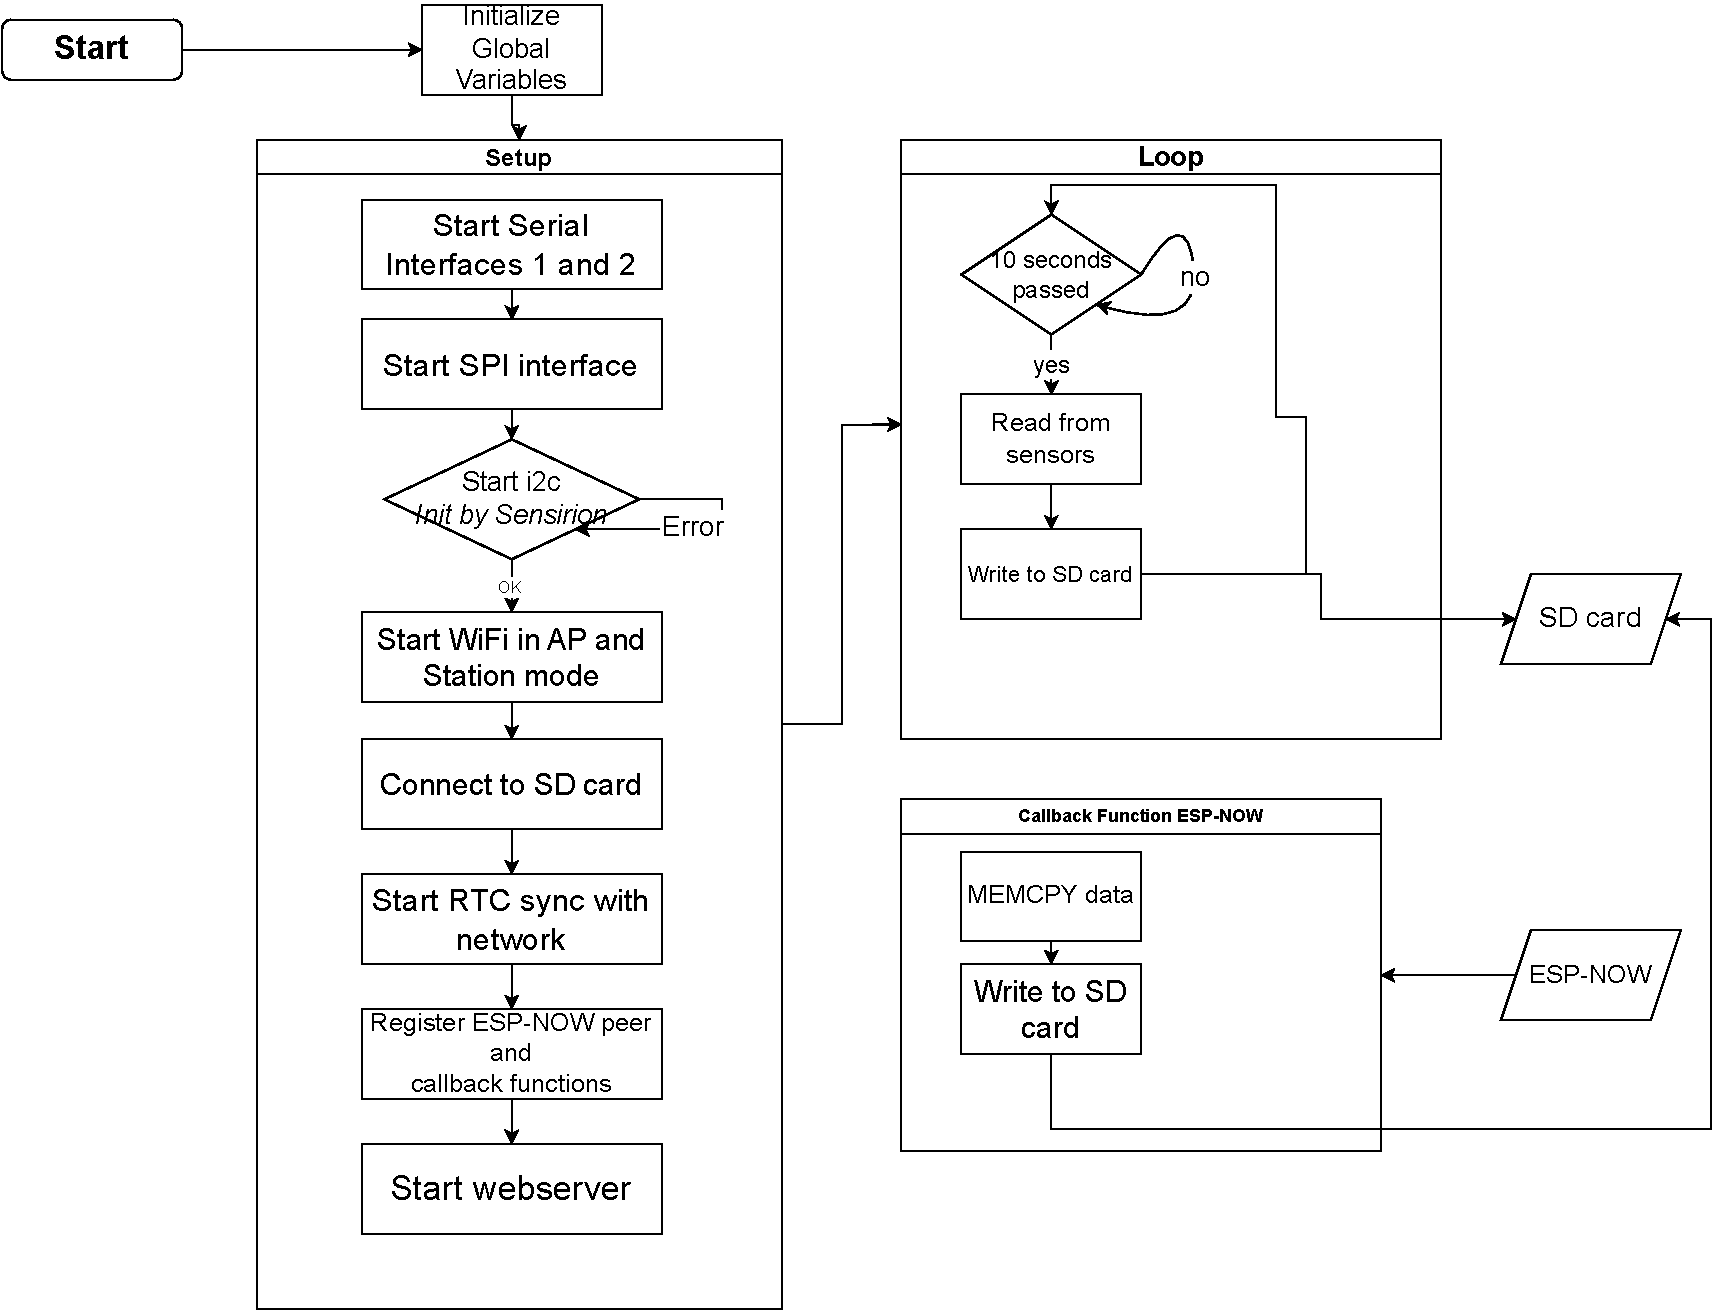
\includegraphics[width=\textwidth]{body/fig/flowchart.drawio.png}
	\caption{Flow diagram of software implementation }
	\label{fig:softwareoverview}
\end{figure}

\subsection{UART}
The GPS unit uses UART Serial commands to send its data to the ESP32. The data received from the GPS module is in the format of NMEA strings. This is the standard format for most gps receivers.\cite{NMEA}
\begin{table}[!htb]
	\resizebox{\textwidth}{!}{%
		\begin{tabular}{|l|l|}
			\hline
			NMEA Sentence & Meaning \\ \hline
			GPGGA & Global positioning system fix data (time, position, fix type data) \\ \hline
			GPGLL & Geographic position, latitude, longitude \\ \hline
			GPVTG & Course and speed information relative to the ground \\ \hline
			GPRMC & Time, date, position, course and speed data \\ \hline
			GPGSA & GPS receiver operating mode, satellites used in the position solution, and DOP values. \\ \hline
			GPGSV & The number of GPS satellites in view satellite ID numbers, elevation, azimuth and SNR values. \\ \hline
			GPMSS & Signal to noise ratio, signal strength, frequency, and bit rate from a radio beacon receiver. \\ \hline
			GPTRF & Transit fix data \\ \hline
			GPSTN & Multiple data ID \\ \hline
			GPXTE & cross track error, measured \\ \hline
			GPZDA & Date and time (PPS timing message, synchronized to PPS). \\ \hline
			150 & OK to send message. \\ \hline
		\end{tabular}%
	}
	\label{tab:nmea}
	\caption{NMEA Sentences and their meanings \cite{GPSSentence}}
\end{table}

\noindent
This data is sent over the uart in comma delimited messages, the uart is set to default to 9600 baud.
The ESP32-S2 has 2 hardware UARTs, one is used for debugging and communication with the device while developing and one for communicating with the GPS module. The first UART is set to 115200 baud and the second to 9600 baud. Each UART is initialized separately and the second UART is passed to the gps encoding library TinyGPS++. The first UART is only called when debugging or notices are needed. It is used to check sending of messages using ESP-NOW for example.


\subsection{i2c}
Both the Sensirion and Senseair sensors make use of the i2c bus to communicate. 

\subsection{ESP-NOW}



